\chapter{Interview Questions}
\label{app:interview-questions}

\textit{\small Note: The following questions were originally asked in Danish. English translations are provided below.}

\section{Welcome and Introduction}
\begin{enumerate}
    \item Hello and thank you for taking the time to meet. My name is Jawad and I study software engineering at AAU Copenhagen. I am working on an exam where I need to interview an experienced developer about how work is conducted as a software developer, and we will spend some time on this. If it's okay with you, I will record the conversation so I can transcribe it afterwards. Is that okay?
\end{enumerate}

\section{Project Experiences}
\begin{enumerate}
    \item First of all, I would like to talk a bit about project experiences. If you were to show a new team member an example of how things are done at your workplace, which project would you choose that you work with? And why that one specifically?
    \item Have you experienced having a project that did not live up to expectations? And if you were to return to that project together with your company, what would you have done differently?
    \item When you look back at all the projects and tasks you have been involved in, what characterizes those that just flow and have really good momentum?
    \item How do you assess whether your project was a success, not only for your goals within development, but also whether it has delivered value in the real world?
\end{enumerate}

\section{Work Methods and Daily Practice}
\begin{enumerate}
    \item How would you describe your approach to development? Is there a specific methodology you use, such as Scrum?
    \item How has it evolved over time? Have there been changes in the way you have worked within Scrum?
    \item Can you tell me about the process from when you receive a task until it reaches the users?
    \item How long are your sprints? Who decides what should be done first?
    \item What is the best thing about your current way of working? And what is most frustrating?
\end{enumerate}

\section{The Team and Collaboration}
\begin{enumerate}
    \item Can you paint a picture of the team for me, who is involved, and what are their roles?
    \item How do you ensure that everyone is pulling in the same direction?
    \item How do you communicate on a daily basis? How much contact do you have with those who actually use the product?
\end{enumerate}

\section{Measurement and Continuous Improvement}
\begin{enumerate}
    \item How do you keep track of whether you are on the right path? Do you track velocity, lead time, or other metrics?
    \item Do you hold retrospectives? Can you give an example of something you have changed based on a retro?
    \item Do you feel that management supports your way of working?
    \item How do you ensure that competencies in the team stay sharp?
\end{enumerate}

\section{Quality and Testing}
\begin{enumerate}
    \item When is a task done for you, what needs to be in place before you say finished?
    \item What do you do to ensure quality along the way?
    \item Can you describe your test approach, which types of tests do you run, and when?
    \item What happens when you find a bug, what is the process from when it is discovered until it is fixed?
\end{enumerate}

\section{AI in Development}
\begin{enumerate}
    \item Have you adopted AI tools for development, Copilot, Claude, Cursor, or similar?
    \item What do you primarily use it for? Has it noticeably changed how you work?
    \item Has management said anything about what you may and may not do with AI in the codebase?
\end{enumerate}

\section{CI/CD and Technical Setup}
\begin{enumerate}
    \item Can you describe the journey from when you push code until it runs in production?
    \item Which tools do you use in your CI/CD setup?
    \item How often do you deploy to production? What happens when something goes wrong?
    \item If you had free hands to improve one thing in your setup, what would it be?
\end{enumerate}

\section{Stakeholders}
\begin{enumerate}
    \item Who do you primarily make the product for? Who are your most important stakeholders?
    \item What happens when different stakeholders have opposing interests?
    \item How do you keep different groups updated on what is happening in the project?
\end{enumerate}

\section{Closing}
\begin{enumerate}
    \item How many years have you been doing software development?
    \item If you were to give advice to someone who has just started, what is important to focus on?
\end{enumerate}

\chapter{Interview Transcript}
\label{app:transcript}

\textit{\small The interview was conducted in Danish. Below is the original transcript.}

\begin{center}
\textsc{Agile Software Engineering Interview}\\
\textsc{AAU København, Autumn 2025}
\end{center}
\smallskip
\noindent\textit{Interviewer:} Jawad | \textit{Subject:} Ahmed Sadiq (Senior Developer, 10 to 12 years experience)\\
\textit{Organisation:} Trade Union (internal development department)
\medskip

\subsubsection*{Velkomst og Introduktion}

\noindent\textbf{[00:00:02] Interviewer:} Hej tak fordi du ville mødes. Jeg hedder Jawad og jeg studerer software engineering på AAU København. Jeg er i gang med en eksamen hvor jeg skal interviewe en erfaren udvikler om hvordan arbejdet foregår som softwareudvikler, og vi skal bruge lidt tid på det her. Hvis det er okay med dig, optager jeg samtalen, så kan jeg skrive den ud bagefter. Er det i orden?

\noindent\textit{[Interviewpersonen accepterer]}

\subsubsection*{Sektion 1: Projekterfaringer}

\noindent\textbf{[00:00:30] Interviewer:} Først og fremmest vil jeg gerne tale lidt om projekterfaringer. Hvis du skal vise et nyt teammedlem et eksempel på hvordan tingene gøres på din arbejdsplads, hvilket projekt vil du vælge som du arbejder med? Og hvorfor lige det?

\noindent\textbf{[00:00:51] Interviewperson:} Hvis jeg skulle vise et nyt teammedlem hvordan vi arbejder, så er det jo meget almindelige tools vi bruger. Vi har nogle udviklingsguides liggende, hvor vi fortæller hvordan man sætter sig ind i det og hvilken måde vi arbejder på.

\noindent\textbf{[00:01:05] Interviewperson:} Måden vi arbejder på er at vi har et Scrum board i Jira, hvor der ligger en masse user stories som man kan tage på, indtil de er færdige. Et nyt teammedlem vil allerede vide hvilken teknologi han arbejder inden for det vil sige .NET.

\noindent\textbf{[00:01:34] Interviewperson:} Det vil sige han skal få sin solution op at køre, og så er det i princippet bare at han går hen og kigger på vores forskellige projekter. Vi har et booking system, vi har et kontosystem og vi har forskellige APIer. Afhængig af hvad den enkelte issue går ud på, så sætter det ham ind i den enkelte løsning.

\noindent\textbf{[00:02:04] Interviewer:} Har du oplevet at du har haft et projekt som ikke levede op til forventningerne? Og hvis du skulle tilbage til det projekt sammen med dit firma, hvad har I så gjort anderledes? Har I haft nogle dårlige oplevelser med den måde arbejdet foregår på i jeres projekter?

\noindent\textbf{[00:02:23] Interviewperson:} Ja, inden for min tid som ny udvikler fik jeg en opgave. Det er en fagforening jeg arbejder for, og der er det vigtigste nogensinde medlemsoptagelse det vil sige hvordan man får et medlem ind.

\noindent\textbf{[00:02:34] Interviewperson:} De ville gerne have at man skulle kunne tilmelde sig en Akasse samtidig. Så jeg skulle lave i et meget gammelt legacy system en lille checkbox, som automatisk kunne sende en mail til Akassen og registrere at brugeren viste interesse i at melde sig ind i kassen.

\noindent\textbf{[00:03:04] Interviewperson:} Problemet var bare at i deres medlemssystem kunne vi ikke sikkerhedsindstillingerne tillod ikke at man kunne sætte den indstilling uden at man var logget på som medlem. Og jeg kunne ikke bare lave testmedlemmer.

\noindent\textbf{[00:03:33] Interviewperson:} Der var login på devmiljøet, der var login på testmiljøet, men der var ikke login på produktionsmiljøet. Det vil sige jeg kunne sagtens udvikle det, jeg kunne teste det, men jeg kunne ikke deploye til produktion.

\noindent\textbf{[00:04:02] Interviewperson:} Det gik tabt efterfølgende. Vi prøvede at presse på for at få fjernet den sikkerhedsindstilling, så vi kunne rette direkte på produktionen. Men så fik vi at vide af den juridiske afdeling at det ikke er tilladt, at vi har den data på den måde.

\noindent\textbf{[00:04:32] Interviewperson:} Jeg brugte måske to uger til en måned på den opgave. I virkeligheden skulle den være dræbt meget længe før den overhovedet kom ind til mig. Der manglede en proces opgaven skulle først igennem jura og godkendelse i forhold til GDPR.

\noindent\textbf{[00:04:48] Interviewperson:} Og så bagefter skulle den igennem dem der bestemmer omkring sikkerhedsindstillinger på medlemssystemet, som ikke er vores det er en tredjepart inden den overhovedet kom ind til mig. Det var et rigtig dårligt projekt.

\noindent\textbf{[00:05:17] Interviewer:} Det giver god mening. Når du kigger tilbage på alle de projekter og opgaver du har været på, hvad kendetegner dem som bare kører og som har en rigtig god flow? Er der nogen principper fra Agile I bruger, eller nogle prioriteringer, noget der gør det nemmere og mere behageligt at arbejde med?

\noindent\textbf{[00:05:30] Interviewperson:} Vi har, inden vi går i gang med et projekt, så kører vi altid refinement. Det vil sige at vi har nogle epics som vi sidder og nedbryder til forskellige user stories. Man sidder og nedbryder hele projektet i mange små ting, sådan så vi kan levere features løbende til forretningen i stedet for at komme med det hele på en gang.

\noindent\textbf{[00:06:00] Interviewperson:} Inden vi overhovedet går i gang, så har der været en breakdown, og vi skal få behovene ud af forretningen, som vi så nedbryder til vores opgaver. Hvis forretningen har gjort deres arbejde godt nok, og vi går ordentligt til refinement, og hver user story har sit eget klare formål, så er det det der gør at man virkelig lykkes med et projekt og bagefter er i stand til at kunne levere det.

\noindent\textbf{[00:06:24] Interviewer:} Er der også andre ting I måler på for eksempel kundetilfredshed? Hvordan vurderer I om jeres projekt var en succes, ikke kun for jeres mål inden for udvikling, men også om det er noget som i den virkelige verden har leveret værdi?

\noindent\textbf{[00:06:48] Interviewperson:} Vi kører en gang efter hvert sprint et review, hvor vi som team reviewer hvad vi har lavet i sprintet om vi lykkedes med det, om det var en succes eller en failure, og hvorfor det muligvis ikke lykkedes, så vi kan lære af det.

\noindent\textbf{[00:07:31] Interviewperson:} Og så inden i teamet kører vi også nogle retroer, hvor vi prøver at finjustere på de ting vi arbejder med og hvordan vi arbejder med dem.

\subsubsection*{Sektion 2: Arbejdsmetoder og Daglig Praksis}

\noindent\textbf{[00:07:48] Interviewer:} Nu vil jeg tale lidt mere om arbejdsmetoder og den daglige praksis. Hvordan vil du beskrive jeres tilgang til udvikling? Er der en bestemt metodologi I bruger, som for eksempel Scrum?

\noindent\textbf{[00:07:50] Interviewperson:} Ja, vi bruger Scrum.

\noindent\textbf{[00:07:59] Interviewer:} Hvordan har det udviklet sig over tiden? Har der været ændringer i den måde I har arbejdet på inden for Scrum, eller har I bare holdt den fra starten?

\noindent\textbf{[00:08:27] Interviewperson:} Vi er ikke helt klassisk Scrum. Vi piller nogle ting fra, fordi vi er en intern udviklingsafdeling. Der er også en masse driftsopgaver som ikke på samme måde kan køre som et projekt. For eksempel fixes du kan ikke køre det som et projekt, du er nødt til at lave det indtil det er færdigt.

\noindent\textbf{[00:08:41] Interviewer:} Er der nogle ting I har ændret ved jeres arbejdsmetode med Scrum over tiden?

\noindent\textbf{[00:08:58] Interviewperson:} Vi har beholdt de ting som giver mening og droppet de ting som ikke giver mening. Vi har for eksempel droppet story points, fordi det var meget udefinerbart hvad de gik ud på.

\noindent\textbf{[00:09:27] Interviewperson:} Det kan godt være at man internt i teamet kunne få en forståelse for hvad de handlede om, men det var meget svært at gøre sådan at kolleger kunne forstå hvad de reelt betød. Vores Scrum master fandt på andre ting hundestørrelser, tshirtstørrelser og alt muligt andet for at gå væk fra tal, fordi når det bare er et tal, så tror man ofte det er dage, og det er det bare ikke.

\noindent\textbf{[00:09:59] Interviewperson:} Vi har også nogle gange droppet en retro hvis det ikke gav mening. Vi har droppet et sprint review fordi man ikke rigtig følte det var et sprint man havde kørt i den periode. Så vi bruger Scrummetoderne, men vi tilpasser dem.

\noindent\textbf{[00:10:22] Interviewer:} Kan du fortælle mig processen der gennemgås når I har fået en opgave? Hvad sker der fra I har fået opgaven til den når ud til brugerne? Hvilke skridt skal I igennem for at opgaven kan blive ført ud i virkeligheden?

\noindent\textbf{[00:10:52] Interviewperson:} Forretningen kommer med en opgave til en product manager. Det er ikke en del af Scrummetoden, det er bare noget for forretningen. Product manageren har et stort Excelark med alle opgaverne.

\noindent\textbf{[00:11:22] Interviewperson:} Forretningen vælger så at give opgaven videre til en Product Owner, der prioriterer det i forhold til resten af sine opgaver. Product Owneren tager eventuelle samtaler med forretningen og brugerne for at få behovene ud hvorfor laver vi det her, og hvad prøver I at få løst?

\noindent\textbf{[00:11:52] Interviewperson:} Når det er gjort, formulerer de nogle epics. En epic kan i princippet være et helt system. Så er det at vi som team bryder hele projektet ned. Vi sidder og splitter det op i user stories.

\noindent\textbf{[00:12:22] Interviewperson:} Så laver vi nogle acceptance criterias hvad er det der skal være opfyldt for at den her feature er færdig? Så kommer den ud på vores backlog. Enten ved sprint start eller undervejs i et sprint tager vi opgaven, og så går vi i gang med at designe det og kode det.

\noindent\textbf{[00:12:52] Interviewperson:} Når det er færdigt, skubber vi det op til Azure DevOps hvor der ligger en pipeline. Den kører nogle tests både enhedstests, integrationstests og endtoend tests. Hvis de alle sammen går igennem, så kan vi lave en pull request ind til mainbranchen.

\noindent\textbf{[00:13:22] Interviewperson:} En kollega skal så godkende pull requesten der skal være en review på koden. Når den er godkendt, merges den ind i main. Fra main kan vi så deploye videre til forskellige miljøer først devmiljø, så testmiljø, og til sidst produktionsmiljøet.

\noindent\textbf{[00:13:52] Interviewer:} Hvor lange er jeres sprints? Har I eksperimenteret med andre længder?

\noindent\textbf{[00:14:07] Interviewperson:} Vi kører tougers sprints. Vi har prøvet tre uger, men det blev for langt. En uge var for kort til at få noget meningsfuldt fra hånden. To uger fungerer godt for os.

\noindent\textbf{[00:14:37] Interviewer:} Hvem bestemmer hvad der skal laves først? Hvordan foregår den prioritering?

\noindent\textbf{[00:14:52] Interviewperson:} Det er Product Owneren der prioriterer i samarbejde med forretningen. De kigger på business value hvad giver mest værdi for organisationen og medlemmerne. De kigger også på dependencies nogle ting skal være på plads før andre kan laves.

\noindent\textbf{[00:15:22] Interviewer:} Hvad er det bedste ved jeres nuværende måde at arbejde på?

\noindent\textbf{[00:15:37] Interviewperson:} Flexibiliteten. Vi kan hurtigt tilpasse os hvis prioriteterne ændrer sig. Og så føler jeg vi har god transparens alle ved hvad der foregår og hvorfor.

\noindent\textbf{[00:15:52] Interviewer:} Og hvad er mest frustrerende i det daglige arbejde?

\noindent\textbf{[00:16:07] Interviewperson:} Nogle gange får vi opgaver der ikke er ordentligt defineret, og så skal vi bruge tid på at finde ud af hvad der egentlig menes. Og så kan legacykoden nogle gange være en udfordring at arbejde med.

\subsubsection*{Sektion 3: Teamet og Samarbejde}

\noindent\textbf{[00:16:37] Interviewer:} Kan du tegne et billede af teamet for mig hvem er med, og hvad er deres roller?

\noindent\textbf{[00:16:52] Interviewperson:} Vi har en Product Owner der prioriterer opgaver og taler med forretningen. Vi har en Scrum Master der sørger for at Scrumprocesserne bliver fulgt og fjerner blokeringer for teamet.

\noindent\textbf{[00:17:22] Interviewperson:} Så har vi udviklingsteamet vi er omkring 5 eller 6 udviklere. Vi har også nogle tech leads der hjælper med de mere tekniske beslutninger og arkitektur.

\noindent\textbf{[00:17:52] Interviewer:} Hvordan sikrer I at alle trækker i samme retning at alle ved hvad der er vigtigt lige nu?

\noindent\textbf{[00:18:07] Interviewperson:} Vi har sprint goals som bliver kommunikeret ved sprint start. Alle ved hvad målet er for det sprint. Vores backlog er transparent alle kan se hvad der skal laves og i hvilken rækkefølge.

\noindent\textbf{[00:18:37] Interviewperson:} Vi har også vores Definition of Done som er klar, så alle ved hvad der skal være på plads før noget er færdigt. Vi holder daily standups hvor alle fortæller hvad de arbejder på og om der er nogle blokeringer.

\noindent\textbf{[00:19:07] Interviewer:} Hvordan kommunikerer I i det daglige standups, Slack, ad hoc møder?

\noindent\textbf{[00:19:22] Interviewperson:} Vi har daily standups hver morgen. Vi bruger Teams til daglig kommunikation og hurtige spørgsmål. Vi har også sprint planning, refinement sessions, reviews og retroer som faste møder.

\noindent\textbf{[00:19:52] Interviewperson:} Og så tager vi selvfølgelig ad hoc møder når der er behov for det hvis der er et større problem eller noget der skal designes.

\noindent\textbf{[00:20:22] Interviewer:} Hvor meget kontakt har I med dem der faktisk bruger produktet?

\noindent\textbf{[00:20:37] Interviewperson:} I sprint reviews inviterer vi nogle gange interessenter fra forretningen til at se hvad vi har lavet. Vi har også kvartalsvise demoer hvor vi demonstrerer for en bredere gruppe hvad vi har udviklet over de seneste tre måneder.

\noindent\textbf{[00:21:07] Interviewperson:} Med medlemmerne har vi ikke direkte kontakt de får nyhedsbreve når der kommer nye features. Product Owneren og forretningen har mere direkte kontakt med medlemmerne og bringer feedback tilbage til os.

\subsubsection*{Sektion 4: Måling og Løbende Forbedring}

\noindent\textbf{[00:21:37] Interviewer:} Hvordan holder I øje med om I er på rette vej? Tracker I velocity, lead time eller andre metrics?

\noindent\textbf{[00:21:52] Interviewperson:} Vi tracker hvor mange opgaver vi får færdige per sprint. Vi kigger også på hvor lang tid det tager fra en opgave starter til den er deployed til produktion.

\noindent\textbf{[00:22:22] Interviewperson:} Vi har også quality metrics hvor mange bugs finder vi, hvor mange kommer tilbage fra produktion. Det giver os en idé om kvaliteten af vores arbejde.

\noindent\textbf{[00:22:52] Interviewer:} Holder I retrospectives? Kan du give et eksempel på noget I har ændret baseret på en retro?

\noindent\textbf{[00:23:07] Interviewperson:} Ja, vi holder retro efter hvert sprint. Et eksempel kunne være at vi fandt ud af at vores code reviews tog for lang tid, fordi folk ikke havde tid til at kigge på dem med det samme.

\noindent\textbf{[00:23:37] Interviewperson:} Så efter retroen aftalte vi at hvis nogen laver en pull request, så skriver de i Teams, og så skal der være nogen der kigger på den inden for 4 timer. Det gjorde at vores flow blev meget bedre.

\noindent\textbf{[00:24:07] Interviewer:} Føler I at ledelsen bakker op om jeres måde at arbejde på? Har I den frihed og de ressourcer I har brug for?

\noindent\textbf{[00:24:22] Interviewperson:} Ja, overordnet set får vi god opbakning. Ledelsen forstår at vi har brug for tid til at gøre tingene ordentligt. Hvis vi siger at noget tager længere tid end forventet, så lytter de.

\noindent\textbf{[00:24:52] Interviewperson:} De prøver også at fjerne blokeringer for os hvis vi mangler adgang til noget eller skal have godkendelser fra andre afdelinger, så hjælper de med det.

\noindent\textbf{[00:25:22] Interviewer:} Hvor gode er I til at skifte retning når kravene ændrer sig?

\noindent\textbf{[00:25:37] Interviewperson:} Det er en af fordelene ved Agile vi kan forholdsvis nemt ændre kurs. Hvis forretningen kommer og siger at prioriteterne har ændret sig, så kan vi tage det op til næste sprint planning og ændre hvad vi arbejder på.

\noindent\textbf{[00:26:07] Interviewperson:} Nogle gange sker det også midt i et sprint, men så prøver vi at undgå det, medmindre det er virkelig kritisk.

\noindent\textbf{[00:26:37] Interviewer:} Hvordan sørger I for at holde kompetencerne skarpe i teamet?

\noindent\textbf{[00:26:52] Interviewperson:} Vi har mulighed for at tage kurser og certificeringer. Vi deler også viden internt hvis nogen har lært noget nyt, så holder de en kort præsentation for resten af teamet. Og så lærer vi meget af hinanden gennem code reviews og pair programming.

\subsubsection*{Sektion 5: Kvalitet og Test}

\noindent\textbf{[00:27:22] Interviewer:} Hvornår er en opgave done for jer hvad skal være på plads før I siger færdig?

\noindent\textbf{[00:27:37] Interviewperson:} Vi har en Definition of Done. Den siger at: Koden skal være skrevet og opfylde acceptance criteria. Der skal være unit tests der dækker den nye kode. Koden skal være code reviewed og godkendt. Integration tests skal køre uden fejl. Det skal være deployed til testmiljø og testet der. Dokumentation skal være opdateret hvis relevant. Product Owner skal have accepteret det.

\noindent\textbf{[00:28:22] Interviewer:} Hvad gør I for at sikre kvaliteten undervejs code review, pair programming, static analysis?

\noindent\textbf{[00:28:37] Interviewperson:} Vi bruger code reviews på alle pull requests mindst én kollega skal godkende før kode merges. Vi bruger ikke så meget pair programming, men nogle gange hvis noget er særligt komplekst eller hvis en junior udvikler skal lære noget.

\noindent\textbf{[00:29:07] Interviewperson:} Vi har også static analysis der kører automatisk i vores pipeline det tjekker for code style issues og potentielle bugs.

\noindent\textbf{[00:29:37] Interviewer:} Kan du beskrive jeres test approach hvilke typer tests kører I, og hvornår?

\noindent\textbf{[00:29:52] Interviewperson:} Vi har flere lag af tests. Unit tests de kører lokalt når vi udvikler og i pipelinen når vi pusher kode. De tester individuelle funktioner og metoder.

\noindent\textbf{[00:30:22] Interviewperson:} Integration tests de kører i pipelinen og tester at forskellige dele af systemet fungerer sammen. Endtoend tests de kører også i pipelinen og simulerer rigtige brugerflows igennem hele systemet.

\noindent\textbf{[00:30:52] Interviewperson:} Nogle gange laver vi også manuel testing på testmiljøet før vi deployer til produktion.

\noindent\textbf{[00:31:22] Interviewer:} Hvor meget af jeres testing er automatiseret? Har I tillid til at tests fanger problemerne?

\noindent\textbf{[00:31:37] Interviewperson:} De fleste af vores tests er automatiseret. Vi har god code coverage med vores unit tests. Men vi stoler ikke 100 procent på dem der kan altid være edge cases vi ikke har fanget.

\noindent\textbf{[00:32:07] Interviewperson:} Så vi laver også manuel testing af nye features inden de går til produktion. Men automatiseringen giver os god tillid til at vi ikke har ødelagt noget eksisterende når vi laver ændringer.

\noindent\textbf{[00:32:37] Interviewer:} Hvad sker der når I finder en bug hvad er processen fra den opdages til den er fixet?

\noindent\textbf{[00:32:52] Interviewperson:} Hvis vi finder en bug i test, så opretter vi en bug ticket i Jira. Den bliver prioriteret af Product Owner hvis det er kritisk, får den høj prioritet og vi fixer den med det samme. Hvis det er mindre vigtigt, kommer den i backloggen.

\noindent\textbf{[00:33:22] Interviewperson:} Hvis der kommer en bug fra produktion, så evaluerer vi hvor alvorlig den er. Hvis det er noget der stopper brugerne, så dropper vi hvad vi har i hænderne og fixer det. Ellers kommer den i backloggen som en prioriteret opgave.

\subsubsection*{Sektion 6: AI i Udviklingen}

\noindent\textbf{[00:33:52] Interviewer:} Har I taget AIværktøjer i brug til udvikling Copilot, Claude, Cursor eller lignende?

\noindent\textbf{[00:34:07] Interviewperson:} Ja, vi bruger GitHub Copilot.

\noindent\textbf{[00:34:22] Interviewer:} Hvad bruger I det primært til? Hvor giver det mest værdi i hverdagen?

\noindent\textbf{[00:34:37] Interviewperson:} Vi bruger det hovedsageligt til code completion når man skriver kode, så foreslår den hvordan resten af funktionen kunne se ud. Vi bruger det til at skrive boilerplate kode og repetitiv kode hurtigere.

\noindent\textbf{[00:35:07] Interviewperson:} Det er faktisk ret godt til at skrive unit tests den kan generere test cases. Og nogle gange bruger vi det til at forklare kompleks kode man ikke helt forstår.

\noindent\textbf{[00:35:37] Interviewer:} Har det ændret noget mærkbart ved hvordan I arbejder?

\noindent\textbf{[00:35:52] Interviewperson:} Ja, det har gjort os hurtigere til visse opgaver. Især den repetitive kode går meget hurtigere. Men man skal stadig vide hvad man laver AIen foreslår ikke altid den bedste løsning, så man skal kunne vurdere om det den foreslår giver mening.

\noindent\textbf{[00:36:22] Interviewer:} Har I oplevet situationer hvor AIgenereret kode har skabt problemer?

\noindent\textbf{[00:36:37] Interviewperson:} Vi har heldigvis ikke oplevet større problemer endnu, men man skal være opmærksom. Koden er ikke altid den bedste. Nogle gange foreslår den løsninger der virker, men som ikke følger vores coding standards eller best practices. Så man skal stadig review koden ordentligt, selvom den kommer fra AI.

\noindent\textbf{[00:37:07] Interviewer:} Har ledelsen sagt noget om hvad I må og ikke må med AI i kodebasen?

\noindent\textbf{[00:37:22] Interviewperson:} Vi har haft nogle diskussioner om det. Hovedreglen er at man stadig er ansvarlig for den kode man skriver, uanset om det er AIgenereret eller ej. Og man skal være forsigtig med ikke at sende følsom forretningskode til eksterne AItjenester.

\noindent\textbf{[00:37:52] Interviewer:} Hvordan ser du AI i fremtiden for jeres arbejdsplads?

\noindent\textbf{[00:38:07] Interviewperson:} Jeg tror AI vil gøre at vi bruger færre udviklere i fremtiden. Men jeg tror ikke det erstatter os helt. Der vil stadig være behov for nogen der forstår forretningen, kan designe løsninger og vurdere om den kode AI genererer faktisk løser problemet ordentligt. AI er et værktøj der gør os mere produktive, men det kræver stadig erfarne udviklere til at guide det og sikre kvaliteten.

\subsubsection*{Sektion 7: CI/CD og Teknisk Setup}

\noindent\textbf{[00:38:37] Interviewer:} Kan du beskrive rejsen fra du pusher kode til det kører i produktion hvilke trin passerer det igennem?

\noindent\textbf{[00:38:52] Interviewperson:} Når jeg pusher kode til Azure DevOps, så bygges koden automatisk. Unit tests kører, integration tests kører, og static analysis kører.

\noindent\textbf{[00:39:22] Interviewperson:} Hvis alt går igennem, kan jeg lave en pull request til main branch. En kollega skal code reviewe og godkende. Når den er godkendt, merges den til main. Fra main kan vi deploye til devmiljø først, så til testmiljø hvor vi tester manuelt, og til sidst til produktion når alt ser godt ud.

\noindent\textbf{[00:39:52] Interviewer:} Hvilke tools bruger I i jeres CI/CD setup GitHub Actions, Jenkins, Azure DevOps eller noget andet?

\noindent\textbf{[00:40:07] Interviewperson:} Vi bruger Azure DevOps til det hele. Det er vores version control system, vores CI/CD platform, der kører vores pipelines og builds. Vi bruger Azure Containers til at køre vores applikationer i skyen. Og vi har logging i Azure portalen, så vi kan se hvad der sker i vores systemer. Det er smart at have det hele i én platform det gør det nemmere at arbejde med.

\noindent\textbf{[00:40:37] Interviewer:} Hvor meget kører automatisk vs. hvor meget kræver manuel godkendelse?

\noindent\textbf{[00:40:52] Interviewperson:} Build og test er fuldt automatisk det starter hver gang nogen pusher kode. Men deployment er delvist manuelt. Vi skal godkende at koden deployes til hvert miljø. Jeg kan ikke bare pushe kode direkte til produktion. Det skal igennem en branch, lave en pull request, få code review, blive godkendt, og så kan vi deploye. Det giver os kontrol og sikkerhed for at forkert kode ikke kommer direkte ud til brugerne.

\noindent\textbf{[00:41:22] Interviewer:} Hvor ofte deployer I til produktion? Er det kontinuerligt, dagligt, ugentligt, eller efter en specifik sprint?

\noindent\textbf{[00:41:37] Interviewperson:} Det varierer meget. Hvis der er noget der bliver færdigt i løbet af et sprint, så bliver det deployed. Når en feature er færdig, skal den selvfølgelig deployes. Vi deployer ofte til udviklings og testmiljøer. Til produktion er det som minimum en gang per sprint cirka, men det kan godt være oftere hvis vi har flere features færdige.

\noindent\textbf{[00:42:07] Interviewer:} Hvad sker der når noget går galt i produktion hvem får alarm, og hvad er processen?

\noindent\textbf{[00:42:22] Interviewperson:} Vi har SMSovervågning sat op. Det vil sige at hvis der er noget kritisk der går galt, får vi SMSalarmer. Hvis det sker om natten, må vi håbe at nogen våger. Ellers opdager vi det om morgenen.

\noindent\textbf{[00:42:52] Interviewperson:} Vi har altid en tidligere version liggende klar. Hvis der går noget alvorligt galt, kan vi rulle tilbage til den forrige løsning hurtigt. Det tager typisk kun få minutter at gå tilbage til en version der virker. Så kan vi i løbet af dagen analysere hvad der gik galt og lave et ordentligt fix.

\noindent\textbf{[00:43:22] Interviewer:} Hvor oplever I de største udfordringer i jeres pipeline?

\noindent\textbf{[00:43:37] Interviewperson:} Nogle gange kan vores tests være ustabile de fejler af og til uden grund og skal bare køres igen. Det kan være frustrerende. Og så kunne vores monitoring være bedre. Vi kunne logge meget mere og have flere alarmer sat op, så vi hurtigere opdager når noget går galt.

\noindent\textbf{[00:44:07] Interviewer:} Hvis du fik frie hænder til at forbedre én ting i jeres setup, hvad ville det være?

\noindent\textbf{[00:44:22] Interviewperson:} Jeg ville forbedre vores logging og monitoring betydeligt. Vi kunne logge meget mere detaljeret information, og vi kunne sætte langt flere alarmer op, så vi proaktivt får besked når noget ser mærkeligt ud i stedet for at vente til systemet går helt ned.

\subsubsection*{Sektion 8: Stakeholders og Omverdenen}

\noindent\textbf{[00:44:52] Interviewer:} Hvem er det I primært laver produktet for? Hvem er jeres vigtigste interessenter?

\noindent\textbf{[00:45:07] Interviewperson:} Det afhænger af hvilket system vi arbejder med. Nogle gange er det internt i forretningen altså vores kollegaer der bruger systemerne. Men medlemmerne er helt klart de primære brugere. De er dem vi ultimativt laver det for. Og så er der selvfølgelig også forretningen og ledelsen som stakeholders.

\noindent\textbf{[00:45:37] Interviewer:} Hvad sker der når forskellige stakeholders har modsatrettede interesser?

\noindent\textbf{[00:45:52] Interviewperson:} Økonomi er helt klart vigtigt. Hvis organisationen siger at noget er for dyrt eller ikke kan lade sig gøre økonomisk, så stopper vi projektet. Hvis forretningsønsker ikke giver mening i forhold til systemet teknisk, så er det os der vinder. Det kan godt være de vil have en knap der blinker, men hvis den knap ødelægger hele systemet, så får de den ikke. Men generelt prøver vi at finde kompromiser hvor alle parter kan få noget af det de vil have, og hvor vi leverer værdi til medlemmerne.

\noindent\textbf{[00:46:22] Interviewer:} Hvordan holder I forskellige grupper opdateret på hvad der sker i projektet?

\noindent\textbf{[00:46:37] Interviewperson:} Internt holder vi kvartalsvise demoer, hvor vi demonstrerer hvad vi har lavet i de seneste tre måneder for forretningen og ledelsen. Medlemmerne får nyhedsbreve når der kommer nye features eller ændringer i systemerne. Vi har ikke direkte kommunikation med medlemmerne det håndteres af andre afdelinger der så bringer feedback til os.

\subsubsection*{Afrunding}

\noindent\textbf{[00:47:07] Interviewer:} Hvor mange år har du været i gang med softwareudvikling?

\noindent\textbf{[00:47:12] Interviewperson:} Det er omkring 10 til 12 år.

\noindent\textbf{[00:47:22] Interviewer:} Hvis du skulle give et råd til nogen som lige er startet hvad er det vigtige man skal fokusere på for at få et godt arbejdsmiljø og kunne fungere godt og levere noget?

\noindent\textbf{[00:47:37] Interviewperson:} Udover at man selvfølgelig skal være god til at løse problemer, så er det måske også en meget god idé at lære at forklare hvad man laver. Det kan være svært nogle gange at forklare tekniske ting til ikketekniske personer, men det er super vigtigt. Lærer man at kommunikere godt, både med kollegaer og med forretningen, så kommer man meget langt.

\noindent\textbf{[00:48:07] Interviewer:} Mange tak for din tid. Hvis det er i orden, må jeg gerne skrive til dig hvis der dukker nogle opfølgende spørgsmål op?

\noindent\textbf{Interviewperson:} Selvfølgelig, det er helt i orden.

\smallskip
\begin{center}\textit{Slut på interview}\end{center}

\chapter{Thematic Analysis of Interview Data}
\label{app:thematic-analysis}

This appendix documents the thematic analysis process applied to Ahmed's interview responses. The analysis followed an inductive approach, allowing themes to emerge organically from the data.

\section{Familiarization and Initial Observations}

During transcript review, several patterns emerged. Ahmed spoke extensively about process adaptation, describing how the team modified standard Scrum practices to fit their organizational context. His narrative about the failed legacy system task revealed the importance of proper requirements validation. The discussion of refinement sessions highlighted how structured preparation prevents problems.

\section{Coding Process}

The transcript was systematically coded, identifying meaningful segments:

\begin{description}[style=nextline, leftmargin=0.8cm, itemsep=2pt]
    \item[Pragmatic Scrum Adaptation] Team dropped story points because stakeholders misinterpreted them as time estimates. Scrum Master experimented with dog sizes and t shirt sizes. They occasionally skip ceremonies when sprints lack meaningful progress (00:08:58).
    \item[Refinement as Prevention] Structured refinement sessions decompose epics into user stories with clear acceptance criteria. When refinement is thorough and business requirements are well articulated, projects succeed (00:05:30).
    \item[Process Gate Failures] The legacy checkbox task failed because it bypassed legal review and third party coordination. Ahmed spent weeks on work that should have been blocked earlier (00:02:23).
    \item[Definition of Done Discipline] Comprehensive DoD: code must pass review, unit tests must cover new code, integration tests must pass, staging deployment and testing must complete, documentation updated, PO acceptance (00:27:37).
    \item[Flexible Sprint Boundaries] Two week sprints provide structure, but team can accommodate critical changes mid sprint. Regular sprint planning allows course correction (00:25:37).
    \item[Pipeline Quality Gates] Azure DevOps pipelines automatically run unit tests, integration tests, and end to end tests. Code cannot merge without passing all gates and receiving colleague approval (00:12:52).
    \item[AI Tool Integration] GitHub Copilot accelerates boilerplate and repetitive code. Developers must still review AI suggestions against coding standards. Tool helps but does not replace judgment (00:34:37).
    \item[Stakeholder Complexity] Multiple stakeholder groups: internal business users, external members, management. Economic constraints often override feature requests. Technical feasibility can veto business wishes (00:45:07).
    \item[Monitoring Limitations] Current monitoring relies on SMS alerts for critical failures. Improved logging and proactive alerting identified as primary enhancement area (00:43:37).
    \item[Communication Skills] Beyond technical ability, explaining technical concepts to non technical stakeholders is crucial for career success (00:47:37).
\end{description}

\section{Theme Construction}

Codes were organized into four major themes through iterative grouping:

\textbf{Theme A: Adaptive Framework Implementation.} The team treats Scrum as a starting point rather than a rigid prescription. When estimation caused confusion, they experimented with alternatives and moved away from numerical estimates. Their willingness to skip ceremonies when they would not add value demonstrates a focus on outcomes over rituals. \textit{Key evidence:} ``Vi har beholdt de ting som giver mening og droppet de ting som ikke giver mening'' (00:08:58).

\textbf{Theme B: Process as Risk Mitigation.} The failed legacy task fundamentally shaped Ahmed's understanding of why process gates exist. The checkbox feature seemed simple but required legal approval, third party coordination, and production environment access. Today, the team's refinement process explicitly addresses such dependencies. \textit{Key evidence:} ``I virkeligheden skulle den være dræbt meget længe før den overhovedet kom ind til mig'' (00:04:32).

\textbf{Theme C: Balancing Autonomy and Control.} The deployment pipeline provides automatic quality enforcement through tests and code review requirements. This creates control without requiring manual intervention for routine situations. However, deployment to production requires explicit approval, maintaining human oversight at critical transitions. \textit{Key evidence:} ``Jeg kan ikke bare pushe kode direkte til produktion'' (00:40:52).

\textbf{Theme D: Continuous Improvement Through Reflection.} Sprint reviews evaluate what was delivered and whether it met expectations. Retrospectives examine how the team worked and identify process improvements. The code review response time improvement illustrates the retrospective process in action. \textit{Key evidence:} ``Så efter retroen aftalte vi at hvis nogen laver en pull request... skal der være nogen der kigger på den inden for 4 timer'' (00:23:37).

\section{Theme Relationships}

\begin{figure}[h]
\centering
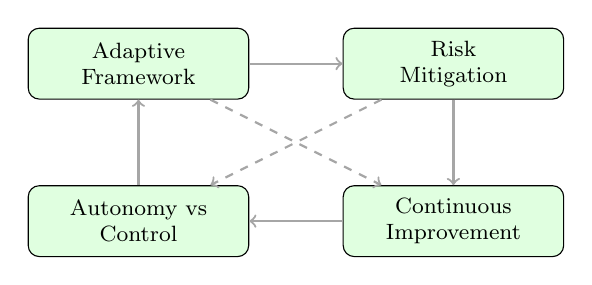
\begin{tikzpicture}[
    box/.style={rectangle, draw=black, fill=green!12, rounded corners, minimum width=2.8cm, minimum height=0.9cm, align=center, font=\footnotesize},
    arr/.style={->, thick, gray!70}
]
\node[box] (adapt) at (0,2) {Adaptive\\Framework};
\node[box] (risk) at (4,2) {Risk\\Mitigation};
\node[box] (balance) at (0,0) {Autonomy vs\\Control};
\node[box] (improve) at (4,0) {Continuous\\Improvement};

\draw[arr] (adapt) -- (risk);
\draw[arr] (risk) -- (improve);
\draw[arr] (improve) -- (balance);
\draw[arr] (balance) -- (adapt);
\draw[arr, dashed] (adapt) -- (improve);
\draw[arr, dashed] (risk) -- (balance);
\end{tikzpicture}
\caption{Theme interconnections in Ahmed's interview}
\label{fig:theme-connections}
\end{figure}

The four themes interconnect significantly. Adaptive Framework Implementation enables Process as Risk Mitigation because the team can modify practices based on what they learn from failures. Balancing Autonomy and Control creates the structure within which Continuous Improvement operates. The retrospective process feeds insights back into framework adaptation.

\section{Summary}

The analysis reveals a trade union development department that has internalized Agile principles while maintaining practical flexibility. Rather than following Scrum literally, they extract value from its practices while adapting to their context as an internal team serving multiple stakeholder groups. Ahmed's perspective, shaped by over a decade of experience including early failures, emphasizes process discipline not as bureaucracy but as protection against avoidable problems.
